\startfirstchapter{Introduction}
\label{chapter:introduction}

Start with 2-3 introductory paragraphs which present the search and summarize the results, as well as how they fit into the wider search for dark matter. 

\section{Introduction to the Standard Model}

The Standard Model (SM) describes all known elementary particles and three of the four known forces by which they interact with one another - the strong, the electromagnetic, and weak forces. The theory of general relativity, which describes the gravitational force, has yet to be incorporated into the SM. 

The known particles, illustrated in Figure \ref{fig:standard_model} are divided into two classes known as ``fermions" and ``bosons" on the basis of an intrinsic form of angular momentum known as ``spin". Fermions carry spin 1/2 and bosons carry integer spin. 

The specific forces by which particles in the SM interact with one another are determined by the charge(s) that they carry. Particles carrying electric charge interact with other particles carrying this charge via the electromagnetic force. Similarly, particles carrying weak and colour charge interact via the weak and strong forces, respectively. 

Each fermion has a corresponding anti-particle with the same mass, but with opposite values of the charges carried - for example, the electron carries negative electric charge and its antiparticle, the positron, carries positive electric charge. 

\begin{figure}[H]
	\centering
	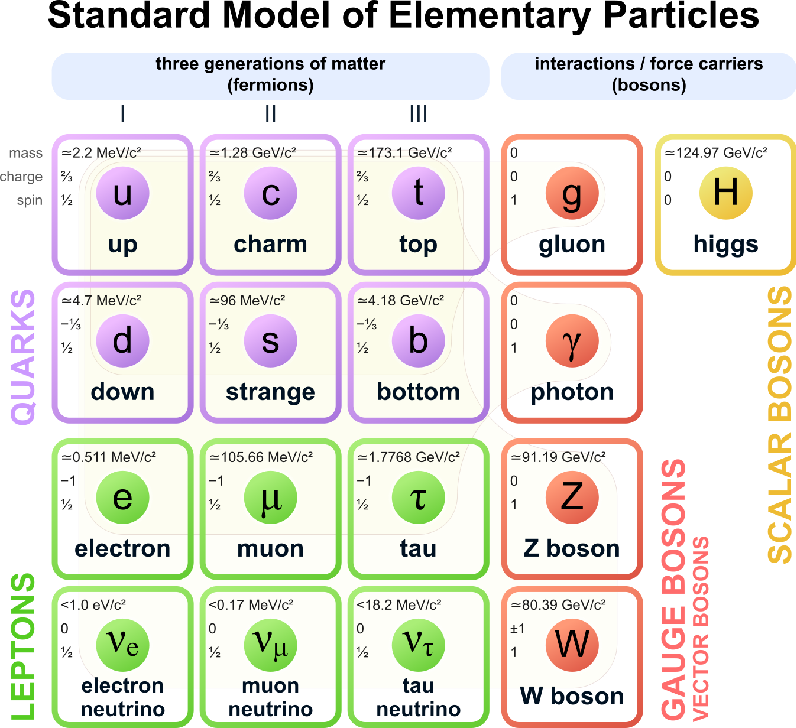
\includegraphics[width=0.7\textwidth]{Figures/1/StandardModel.pdf}
	\caption[]{Names and fundamental properties of particles in the Standard Model}
	\label{fig:standard_model}
\end{figure}

\subsection{Fermions}

Fermions are further sub-divided into leptons and quarks, depending on the charges they carry, and hence the forces by which they interact. There are three known generations of fermions, labelled I, II and III in Figure \ref{fig:standard_model}, each with significantly higher mass than the last. Each generation contains a pair of quarks and a pair of leptons, along with their associated antiparticles. The quark pair consists of one ``up-type" quark with positive electric charge and one ``down-type" with negative charge. The lepton pair consists of one charged lepton and one charge-neutral ``neutrino". 

Leptons carry electric charge and weak isospin, and as a result interact with one another and with other particles carrying these charges via the electromagnetic and weak forces, respectively.  

Quarks also carry electric charge and weak isospin, and additionally carry colour charge. The colour charge allows quarks to interact via the strong force, such that quarks interact by all three forces described by the SM. Unlike charged leptons, which carry an electric charge of \(\pm1\), quarks carry fractional electric charged; up-type quarks carry a charge of \(+\frac{2}{3}\) and down-type carry a charge of \(-\frac{1}{3}\).

Due to an effect known as ``colour confinement", quarks cannot exist as stable particles in isolation, and must instead combine with other quarks to form stable ``colour-neutral" states called ``hadrons". The two major forms of hadrons are ``mesons" formed by a quark-antiquark pair and ``baryons" formed by three quarks. Due to the strength of the strong interaction, there is a relatively high probability that particle production and decay initiated by high energy $pp$ collisions at the LHC will proceed via strong force interactions compared with other forces. As a result, the vast majority of decay products observed in the ATLAS detector are cascades of hadronic interactions in the calorimeter referred to as ``jets" \footnote{See Section \ref{sec:had_calo} for a more detailed discussion of jets in the hadronic calorimeter.} which are initiated by hadrons produced in the collisons.

\subsection{Bosons}

Bosons in the SM are divided into ``gauge bosons" and ``scalar bosons". The gauge bosons are spin 1 force carriers which mediate interactions between particles. The photon mediates electromagnetic interactions between electrically charged particles. The gluon mediates the strong interaction between quarks. Unlike photons which are charge-neutral, the gluon itself carries colour charge, which allows it to self-interact via the strong force. The weak force is mediated by three particles: the electrically neutral Z boson, and two W bosons (W$^\pm$) with opposite electric charges of $\pm$1. 

Scalar bosons are defined as spin 0 particles. There is only one known scalar boson in the SM, namely the Higgs boson (or, simply, the ``Higgs"). Particles in the SM acquire mass via their interaction with the Higgs field. As such, the Higgs only interacts with massive SM particles, which includes all particles except the photon and the gluon. The more massive the particle, the greater its interaction strength - i.e. probability of interaction - with the Higgs. Neutrinos are a possible exception; there is at present no mechanism in the SM by which neutrinos could interact with the Higgs field, so the origin of their tiny masses remains an open question.  

\subsection{Particle Decay and Lifetime}

The lowest-mass ``first-generation" quarks and leptons that comprise column I in Figure \ref{fig:standard_model} and the massless photons and electrons are the only stable particles in the SM. All other particles are unstable, and will decay to less-massive particles after they are produced. The length of time which elapses before an unstable particle decays is determined by the 

The lifetime of an unstable particle quantifies the average length of time 

\subsection{Particle Production and Decay at Colliders}

The LHC is designed to collide protons at a sufficiently high energy that the colliding proton constituents, known as ``partons"\footnote{See section \ref{sec:parton_model} for an introduction to the parton model.}, can pair annihilate to form massive particles. If the massive particles formed by these energetic pair annihilations are 

\begin{itemize}
\item Also take this opportunity to clearly introduce SM details particularly relevant to search
\item Include a discussion of real vs. virtual particles, and on- vs. off-shell production.
\item Hard scatter ME and PS
\item intereference
\end{itemize}

\section{Evidence for Dark Matter from Observational Astronomy and Cosmology}

\begin{itemize}
\item Selection of some particularly interesting/compelling lines, eg. galactic rotation curves, BBN, CMB anisotropies.
\item Propose to avoid going into much detail since this topic is better covered elsewhere. 
\end{itemize}

\section{Dark Matter Composition Hypotheses}

\begin{itemize}
\item Briefly acknowledge the presence of theories which propose non-particle DM or DM as a SM particle (eg. MOND, primordial black holes).
\item Present evidence in favour of the more widely accepted hypothesis that DM is a fundamental BSM particle.
\item Describe what would be gained from an experimental detection/measurement of DM
\begin{itemize}
\item Solidify the case for particle DM.
\item Measure the particle properties of DM which can't be inferred from astronomical observations - mass, interaction mechanisms with SM particles, potential interactions with other BSM particles.
\end{itemize}
\end{itemize}

\section{Dark Matter Search Strategies}
\begin{itemize}
\item Briefly introduce direct and indirect detection approaches and their relative merits
\item More detailed intro to the collider search approach and how it complements the other search modes
\begin{itemize}
\item Sharp lower bound on accessible DM masses suffered by direct detection searches due detector noise threshold is not an issue for collider searches. Neither is the neutrino floor.
\item Possibility to tailor searches to specific hypothetical DM production models by tuning selections $\rightarrow$ emphasize this point, since it's important for this search.
\item If evidence for DM found by any method (collider or otherwise), colliders can offer a superior means of pursuing dedicated measurements of its properties compared with other search modes.
\end{itemize}
\end{itemize}

\subsection{Searching for Dark Matter at Particle Accelerators}

\begin{itemize}
\item Give an idea of the breadth of accelerator DM search program.
\begin{itemize}
\item Resonance searches
\item mono-X searches
\item Model-independent and model-dependent approaches $\rightarrow$ briefly present range of model completeness, from EFT through simplified to complete.
\item Cover searches at hadron and $e^+e^-$ colliders and fixed target experiments.
\end{itemize}
\item Discuss the relative merits of searching for simplified models (bridge gap between EFT and complete theories, avoid overtuning problems inherent with complete models, facilitate adequate coverage of plausible DM production processes).
\item Briefly introduce the Dark Higgs model, and clearly identify it as a simplified model (details to be fleshed out in Chapter 2) $\rightarrow$ emphasize that this search is sensitive to heavy DM ($\gtrsim$60 GeV), with the requirement that $m_\chi>\frac{1}{2}\ms$ (to prevent the $s\rightarrow\chi\chi$ decay mode).
\end{itemize}

